\chapter{DRIPPING FAUCET}
\label{chap:dripping_faucet}
\mquote{not selectet yet}{...}
    In the previous chapter, we discussed the possibility of swapping a complex and often computationally demanding model for a simpler alternative that behaves similarly. Because the accretion disk is an incredibly complex system, we must also follow this approach and find a suitable and computationally manageable simplification. We chose to employ a relatively simple model of a dripping faucet, which is a reasonably well-understood system known to exhibit non-linear behavior under certain conditions. There are two types of dripping faucet models. 

    For a better understanding of drop formation processes and a more detailed study of fluid behavior, we can construct a model based on Navier-Stokes equations or Lagrange equations. The key roles in such a model, which is referred to as \emph{Fluid Dynamical Model} (FDM), are played by surface tension, viscosity, and gravity \cite{faucet1998}.   

    The second type of dripping faucet model is called \emph{Mass-Spring Model}, and as its name suggests, it is based on the approximation of the forming drop as a mass hanging on a spring \cite{shaw1984}. It evolves through time, with the steady fluid influx, until it reaches a predefined critical mass. At that moment, part of the drop is separated, the system resets its parameters, and the cycle repeats. 

    Both types are highly sensitive to the amount of fluid that steadily flows in. This parameter is the determining factor of the non-linear behavior of these systems. Depending on the concrete value of inflow, the dripping intervals can be either periodic or get through period-doubling stages to complete aperiodicity. 

\section{Drop equilibrum states}
    As a prerequisite for dynamical fluid simulations, we need to know the static equilibrium states of hanging drops on a faucet and evaluate the stability of different shapes and sizes. 

    Let us assume a statically hanging axisymmetrical drop with homogenous fluid density $\rho$. According to \cite{faucet1998}, the drop in equilibrium is defined as follows. The pressure inside the drop is 
    
    % 4.2
    \begin{equation}
        P = \rho g z
    \end{equation}

    where $z$ represents the vertical coordinate, and $g$ is gravitaional acceleration. The following expression describes the pressure difference between the inside and outside of the drop

    % 4.3
    \begin{equation}
        P = \Gamma \left( \frac{1}{R_1} + \frac{1}{R_2}  \right),
    \end{equation}

    where the surface tension is represented by $\Gamma$. $R_1$ and $R_2$ are the curvature radii of the drop's surface that, for the axisymmetric drop, are

    % 4.5
    \begin{align}
    \begin{split}
        \frac{1}{R_1} &= - \frac{\diff \theta}{\diff s}, \\
        \frac{1}{R_2} &= \frac{\cos \theta}{r}.
    \end{split}    
    \end{align}

    Figure \ref{fig:drop_equilibrum_definition} explains in detail the variables used to calculate the shape of the hanging drop.
    
    \begin{figure}[H]
    \begin{center}
        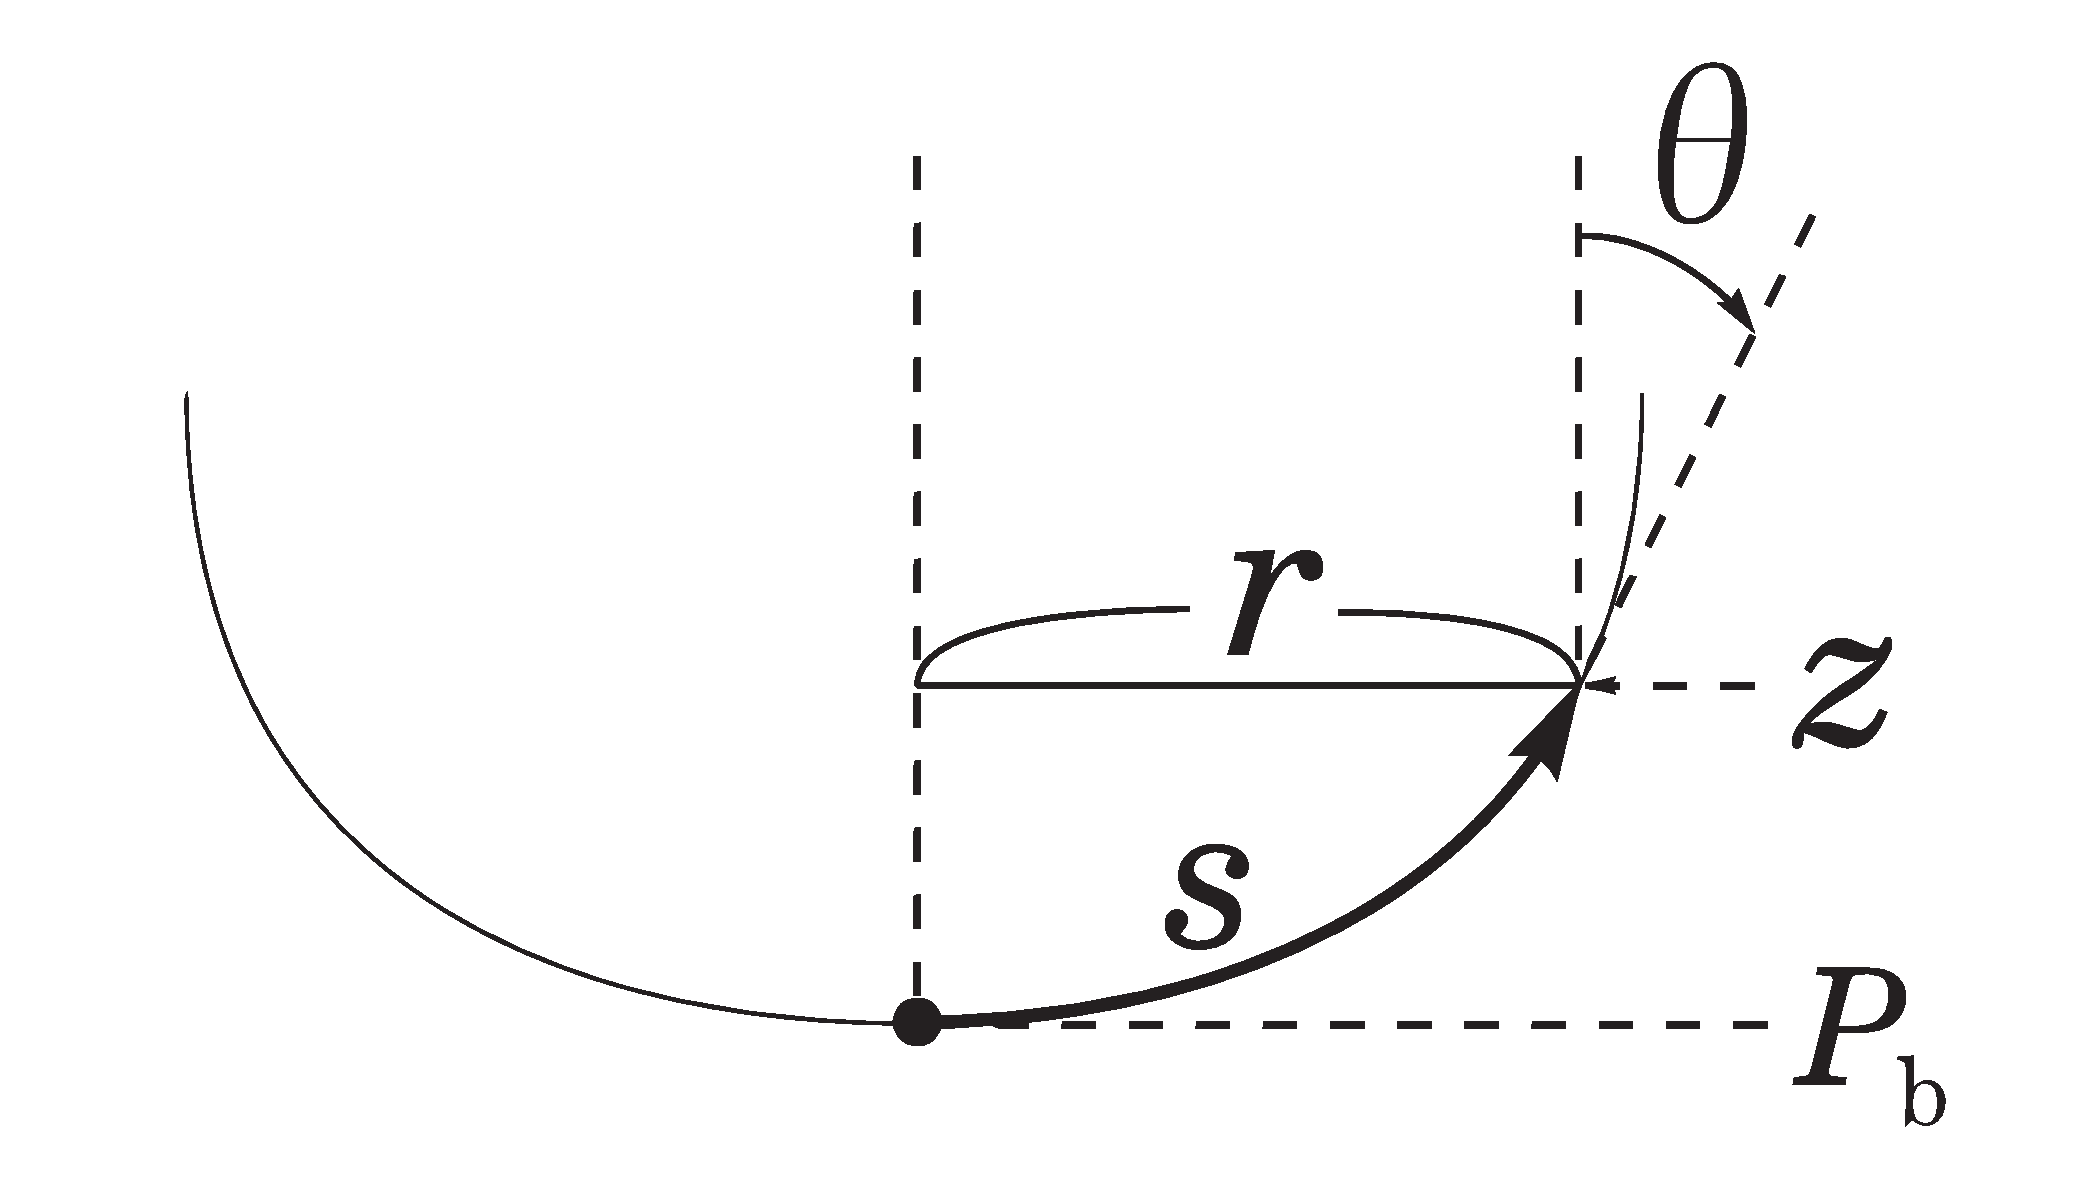
\includegraphics[width=0.75\columnwidth]{img/drop_equilibrum_definition.pdf}
    \end{center}
    \caption{Definition of variables for the hanging drop system. Taken from \cite{faucet1998}} 
    \label{fig:drop_equilibrum_definition}
    \end{figure}

    % 4.4
    \begin{align}
    \begin{split}
        m_0 &= \rho l_0^3 = 0.02 \si{\gram}, \\
        P_0 &= \sqrt{\rho g \Gamma} = 270 \si{dyne \cdot \cm^{-2}}, \\
        l_0 &= \sqrt{\frac{\Gamma}{\rho g}} = 0.27 \si{\cm}, \\
        t_0 &= 0.017 \si{\second}.
    \end{split}
    \label{eq:base_units_drop}
    \end{align}

    Defined by equations \ref{eq:base_units_drop} are the base units of mass, pressure, and length, that sets $\Gamma = \rho = g = 1$; assuming the medium is water at $20 \si{\celsius}$. The drop's shape is then described by a set of ODE's \eqref{eq:drop_equilibrum_odes}, that are solved numerically, with the use of the initial conditions: $z(0) = P_{\mathrm{b}}$, $\theta(0) = \pi / 2$, and $r(0) = 1 \cdot 10^{-20}$

    % 4.6
    \begin{align}
    \begin{split}
        \frac{\diff r}{\diff s} &= \sin \theta, \\
        \frac{\diff z}{\diff s} &= - \cos \theta, \\
        \frac{\diff \theta}{\diff s} &= \frac{ycos \theta}{r} - z.
    \end{split}
    \label{eq:drop_equilibrum_odes}
    \end{align}


\section{Fluid dynamical model (FDM)}

\section{Mass-spring model (MSM)} \label{section:msm}
    \begin{align}
    \begin{split}
        \D{}{t} \left(m \D{z}{t}\right) &= -kz - \gamma\D{z}{t} + mg, \\
        \D{m}{t} &= Q,
    \end{split}
    \label{eq:msm_original_odes}
    \end{align}
    %
    % where $z$ represents the position of the hanging mass $m$. $Q$ is \emph{mass influx}, and it is the main determining parameter of MSM because by choosing a specific value of $Q$, we can drastically alter our model's behavior, as shown in \cite{msmm1999}. Parameter $\gamma=0.05$ is the dampening ratio, and $k$ is the stiffness of the imaginary spring defined as
    %
    \begin{equation}
        \begin{aligned}
            & k~=
            \begin{cases}
                -11.4\ m + 52.5 \hspace{10mm} (m < 4.61) \\
                \hspace{12mm} 0 \hspace{20mm} (m \ge 4.61 ).
            \end{cases}
        \end{aligned}
        \label{eq:spring_stiffness}
    \end{equation}
    %
    % Relations expressed by \eqref{eq:spring_stiffness} and the value of $\gamma$ were obtained experimentally by \cite{shaw1984} and provide a good description for the real-world behavior of drops and leaky faucet. Simply put, \eqref{eq:spring_stiffness} means that if the mass contained in the MSM exceeds the value of $m = 4.61$, the matter essentially goes into free fall.

    \begin{equation}
        z_c = 5.5.
        \label{eq:z_critical_model}
    \end{equation}

\section{Dripping handrail models}











